%-------------------------------------------------------------------------------
% Kyle Westfall
% westfall@ucolick.org
% UCO/Lick Observatory
% University of California, Santa Cruz
% 1156 High St.
% Santa Cruz, CA 95064
% USA
%
% SUBMITTED: 3 Jan 2019
%-------------------------------------------------------------------------------

\documentclass[onecolumn,floatfix,tighten]{aastex62}

\bibliographystyle{aasjournal}

% Units
%\input{shorthands}

% Some fancy commenting
\definecolor{todo}{RGB}{200,0,0}
\newcommand{\comment}[2][todo]{{\color{#1}[[{\bf #2}]]}}

\received{}
\revised{}
\accepted{}
\submitjournal{AJ}

%\shortauthors{Westfall et al.}
%\shorttitle{SDSS-IV/MaNGA Data Analysis Pipeline: Overview}

\begin{document}

\title{ FIDDLES: Fibers in DEIMOS demonstrating light extraction and stability }

%\correspondingauthor{Kyle B. Westfall}
%\email{westfall@ucolick.org}
%
%\author[0000-0003-1809-6920]{Kyle B. Westfall}
%\affiliation{University of California Observatories, University of California, Santa Cruz, 1156 High St., Santa Cruz, CA 95064, USA}

\section{Motivation}

We want to test the performance of coupling of a fiber imaging system to
the focal plane of a slow (f/15) telescope in preparation for building
FOBOS for Keck.

Originally we proposed to do this by constructing and testing a
test-bench assembly at UCO and then designing a system that can be
slotted into the mask holder in DEIMOS. However, there will be very
limited time that we can perform this experiment at Keck, and we
would like to have observations from another telescope as a relative
comparison; e.g., how much does our understanding of the focal plane
affect our ability to couple fibers to it. APF would be good for
this, if we can get some engineering time on it.

\section{Signal-to-Noise Calculation}

I have done some initial S/N calculations for the fiber near-field
profile as measured by FIDDLES mounted on both Lick/APF and
MaunaKea/Keck.

\bigskip

\noindent {\bf Inputs \& Assumptions:}

\begin{itemize}

\item For the source, I use a reference spectrum with a constant AB
magnitude (i.e., constant $F_\nu$) normalized to a given $g$-band
magnitude. I adopt the "no atmosphere" response functions for the
$g$-band filter for sDSS taken from
\url{http://www.sdss.org/wp-content/uploads/2017/04/filter_curves.fits}.

\item I assume we take both on- and off-source (sky-only)
observations, where the source is a point source with a Gaussian
point-spread function. These could be dithered or simultaneous;
however, I have also assumed that I can perfectly subtract the
off-source flux from the the on-source observation (see below).

\item The Maunakea sky spectrum is approximated by taking an observed
dark-sky spectrum observed by MaNGA and rescaling it to match a
DEIMOS dark-sky spectrum over the same wavelength range. The dark-sky
surface brightness of the spectrum is $\mu_g$ = 22.14 mag/arcsec$^2$.

\item For bright-sky conditions, I just scale the dark-sky spectrum
up by 3 mag. This is not correct in that the bright-sky spectrum is
certainly {\bf not} just a scaled up version of the dark-sky
spectrum. However, this was the simplest thing to do for now. Scaling
up by 3 mag may also be a bit extreme.

\item I adopt the Maunakea atmospheric transmission curve used in the
IDL-based Keck ETCs.

\item I adopt the same sky emission and attenuation for both Lick and
Maunakea; light pollution is more significant at Lick meaning that
the S/N estimates at Lick are likely overestimates, at least in dark
conditions.

\item I assume the FIDDLES system performs identically at APF and
Keck.

\item I assume the fiber perfectly scrambles the light in the output
near-field.

\item I assume the off-source near-field image can be perfectly
subtracted from the on-source image.

\item I assume there is no scattered light in the system.

\item The telescope properties relevant to the calculation that I
assumed are in Table 1. The telescope-specific and generic properties
of FIDDLES are provided in Table 2.

\item I assume microlens foreoptics convert the telescope f/15 beam
to f/3 for input to the fiber, that there are no coupling losses, and
that there is no focal-ratio degradation.

\item The fiber attenuation is taken from a WFOS spreadsheet with a
10m fiber run of a Polymicro fiber.

\item I assume the near-field image is a perfectly in focus with no
image-quality degradation by the imaging optics or camera.

\item I use the measurements of the detector properties provided by
Molly for the test-bench camera.

\item I adopt the quantum efficiency curves from
\url{https://www.thorlabs.com/newgrouppage9.cfm?objectgroup_id=7900}
for their 4-megapixel monochrome camera.

\end{itemize}

\noindent {\bf S/N calculation comments:}
\begin{itemize}

\item The detector QE and filter are killer efficiency hits. We
probably don't care for this experiment, though. I thought
astro-grade detectors had efficiencits of more like 90\%, and it's
worth noting Thorlabs has filters that are ~400 \AA wide, but with
peak efficiencies of $\sim$75\%.

\item There is enough overlap between Keck and APF in the S/N plots
that we could feasibly observe the same stars in both (albeit with
the Keck observation at much higher S/N at fixed $m_g$.)

\end{itemize}

\noindent {\bf Considerations for development of FIDDLES and observing plan:}

\begin{itemize}

\item We want to directly measure the point-spread function during
the observations.

\item We want to measure both the near and far-field output of the
fiber; these S/N calculations are for the near-field only. I have not
tried to simulate the far-field.

\item We want to observe with different angles with respect to the
moon to estimate scattered-light effects.

\item We need to consider how differential atmospheric refraction may
affect the observations (e.g., acquisition and guiding).

\end{itemize}

%\section{Details of the experiment}
%
%\subsection{System}
%
%\subsection{Lab calibration}
%
%\section{On-sky tests}

%\input{authors}

%\bibliography{master}

%%%%%%%%%%%%%%%%%%%%%%%%%%%%%%%%%%%%%%%%%%%%%%%%%%%%%%%%%%%%%%%%%%%%%%%%
\begin{deluxetable}{ l c c}
%\tabletypesize{\scriptsize}
\tablewidth{0pt}
\tablecaption{Telescope Properties}
\tablehead{ & \colhead{APF} & \colhead{Keck} }
\startdata
Effective Area (m$^2$)   &  4.47 & 72.37 \\
Plate Scale (mm/arcsec)  & 0.175 &  0.725 \\
Focal Ratio              & 15    &  15
\enddata
\label{tab:properties}
\end{deluxetable}
%%%%%%%%%%%%%%%%%%%%%%%%%%%%%%%%%%%%%%%%%%%%%%%%%%%%%%%%%%%%%%%%%%%%%%%%

%%%%%%%%%%%%%%%%%%%%%%%%%%%%%%%%%%%%%%%%%%%%%%%%%%%%%%%%%%%%%%%%%%%%%%%%
\begin{deluxetable}{ l c c}
%\tabletypesize{\scriptsize}
\tablewidth{0pt}
\tablecaption{FIDDLES Properties}
\tablehead{Property & & }
\startdata
Readnoise (e$-$)         & \multicolumn{2}{c}{6.45} \\
Dark Current (e$-$/s)    & \multicolumn{2}{c}{5} \\
Full-Well (e$-$)         & \multicolumn{2}{c}{18133} \\
Pixel size ($\mu$m)      & \multicolumn{2}{c}{7.4} \\
Fiber diameter ($\mu$m)  & \multicolumn{2}{c}{150} \\
IO Focal Ratio           & \multicolumn{2}{c}{3} \\
\hline
& \colhead{APF} & \colhead{Keck} \\
\hline
Pixel scale (arcsec/pixel) & 0.212 & 0.051 \\
Fiber diameter (arcsec)    & 4.30 & 1.03 \\
Aperture Efficiency ($0\farcs8$ seeing)       & 1.0 & 0.69 \\
\enddata
\label{tab:fiddles}
\end{deluxetable}
%%%%%%%%%%%%%%%%%%%%%%%%%%%%%%%%%%%%%%%%%%%%%%%%%%%%%%%%%%%%%%%%%%%%%%%%

%%%%%%%%%%%%%%%%%%%%%%%%%%%%%%%%%%%%%%%%%%%%%%%%%%%%%%%%%%%%%%%%%%%%%%%%
\begin{figure}
\begin{center}
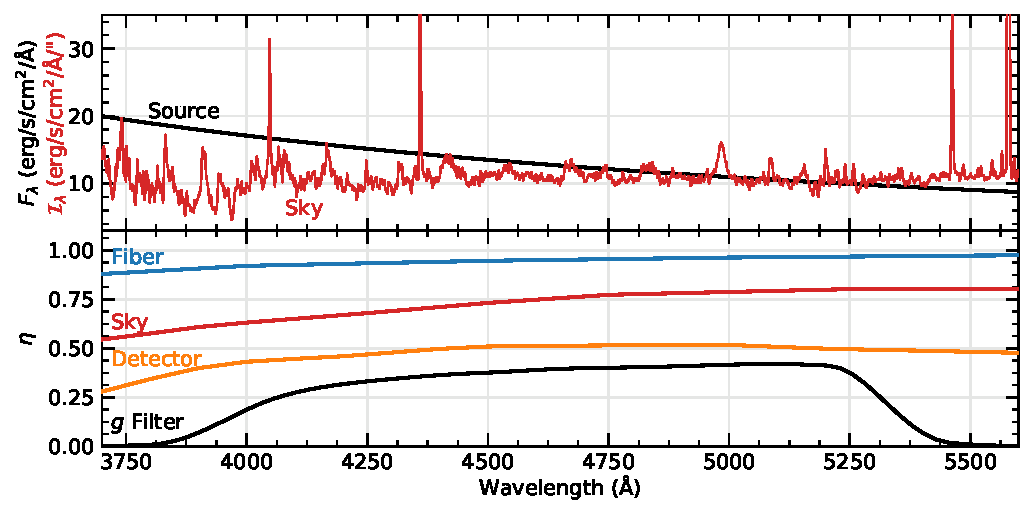
\includegraphics[width=0.9\textwidth]{fiddles_etc_elements.pdf}
\end{center}
\caption{Example components of the S/N calculation. {\it Top} --- The
surface brightness of the sky after artificially scaling up a
dark-sky spectrum by 3 $g$-band magnitudes (red) and the reference
spectrum (constant $F_\nu$) with $m_g = 18$ used to describe the
spectrum of the source. {\it Bottom} --- The effeciency of various
components of the observation, including the fiber (blue), sky (red),
detector quantum efficiency (orange) and $g$-band filter.}
\label{fig:spectra}
\end{figure}
%%%%%%%%%%%%%%%%%%%%%%%%%%%%%%%%%%%%%%%%%%%%%%%%%%%%%%%%%%%%%%%%%%%%%%%%

%%%%%%%%%%%%%%%%%%%%%%%%%%%%%%%%%%%%%%%%%%%%%%%%%%%%%%%%%%%%%%%%%%%%%%%%
\begin{figure}
\begin{center}
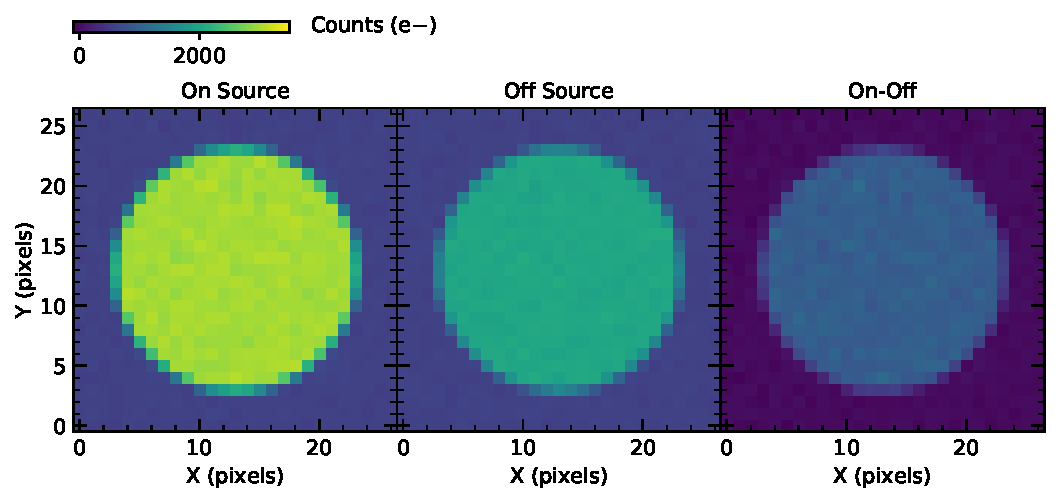
\includegraphics[width=0.9\textwidth]{fiddles_etc_realization.pdf}
\end{center}
\caption{Example realization of the output near-field image both on
(left) and off (middle) the point source, as well as the difference
between the two (right). The S/N calculations provide the S/N per
pixel in the brightest part of the right image. The realization is
for an 18th magnitude star observed by Keck under bright conditions,
directly comparable to the data provided in Figure 3.}
\label{fig:images}
\end{figure}
%%%%%%%%%%%%%%%%%%%%%%%%%%%%%%%%%%%%%%%%%%%%%%%%%%%%%%%%%%%%%%%%%%%%%%%%


%%%%%%%%%%%%%%%%%%%%%%%%%%%%%%%%%%%%%%%%%%%%%%%%%%%%%%%%%%%%%%%%%%%%%%%%
\begin{figure}
\begin{center}
\includegraphics[width=0.45\textwidth]{fiddles_etc_dark.pdf}
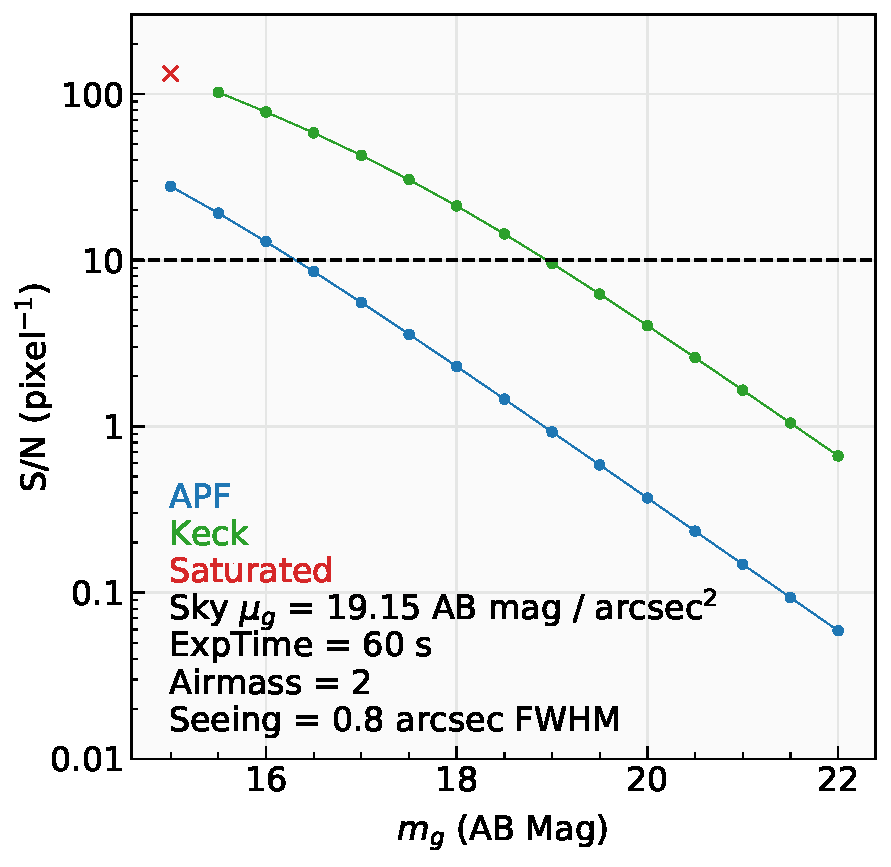
\includegraphics[width=0.45\textwidth]{fiddles_etc_bright.pdf}
\end{center}
\caption{S/N estimates in the brightest part of the near-field
difference image (see Figure 2) as a function of point source
$g$-band magnitude; the left panel assumes dark sky conditions,
whereas the right panel artificially amplifies the dark-sky spectrum
by 3 magnitudes. Results are shown for both APF (blue) and Keck
(green) observations; the observation of the 15th magnitude star at
Keck should saturate the current test-bench detector in a 60 second
integration.}
\label{fig:snr}
\end{figure}
%%%%%%%%%%%%%%%%%%%%%%%%%%%%%%%%%%%%%%%%%%%%%%%%%%%%%%%%%%%%%%%%%%%%%%%%



\end{document}

